\documentclass[a4paper]{article} 
\addtolength{\hoffset}{-2.25cm}
\addtolength{\textwidth}{4.5cm}
\addtolength{\voffset}{-3.25cm}
\addtolength{\textheight}{5cm}
\setlength{\parskip}{0pt}
\setlength{\parindent}{0in}

%----------------------------------------------------------------------------------------
%	PACKAGES AND OTHER DOCUMENT CONFIGURATIONS
%----------------------------------------------------------------------------------------
\usepackage{bm} % Bold math symbols, !must be loaded before unicode-math!
\usepackage{blindtext} % Package to generate dummy text
\usepackage{enumerate} % Enumerate with redefinable labels
\usepackage{enumitem} % Enumerate with redefinable labels
\renewcommand{\thesubsection}{\thesection.\alph{subsection}} % Enumerate subsections with letters
\renewcommand{\thesubsubsection}{\thesubsection.\roman{subsubsection}} % Enumerate subsubsections with roman numerals
\usepackage{charter} % Use the Charter font
\usepackage[utf8]{inputenc} % Use UTF-8 encoding
\usepackage{microtype} % Slightly tweak font spacing for aesthetics
\usepackage[english, ngerman]{babel} % Language hyphenation and typographical rules
\usepackage{amsthm, amsmath, amssymb} % Mathematical typesetting
\newcommand{\argmax}[1]{\underset{#1}{\text{arg max}}\;}
\newcommand{\argmin}[1]{\underset{#1}{\text{arg min}}\;}
\newcommand{\mb}[1]{\mathbf{#1}}  % Bold math symbols shorthand
\usepackage{float} % Improved interface for floating objects
\usepackage[final, colorlinks = true, 
            linkcolor = black, 
            citecolor = black]{hyperref} % For hyperlinks in the PDF
\usepackage{graphicx, multicol} % Enhanced support for graphics
\usepackage{xcolor} % Driver-independent color extensions
\usepackage{marvosym, wasysym} % More symbols
\usepackage{rotating} % Rotation tools
\usepackage{censor} % Facilities for controlling restricted text
\usepackage{listings, style/lstlisting} % Environment for non-formatted code, !uses style file!
\usepackage{pseudocode} % Environment for specifying algorithms in a natural way
\usepackage{style/avm} % Environment for f-structures, !uses style file!
\usepackage{booktabs} % Enhances quality of tables
\usepackage{tikz-qtree} % Easy tree drawing tool
\usepackage{todonotes} % Tool to insert TODOs
\tikzset{every tree node/.style={align=center,anchor=north},
         level distance=2cm} % Configuration for q-trees
\usepackage{style/btree} % Configuration for b-trees and b+-trees, !uses style file!
\usepackage[backend=biber,style=numeric,
            sorting=nyt]{biblatex} % Complete reimplementation of bibliographic facilities
% \addbibresource{ecl.bib}
\usepackage{csquotes} % Context sensitive quotation facilities
\usepackage[yyyymmdd]{datetime} % Uses YEAR-MONTH-DAY format for dates
\renewcommand{\dateseparator}{-} % Sets dateseparator to '-'
\usepackage{fancyhdr} % Headers and footers
\pagestyle{fancy} % All pages have headers and footers
\fancyhead{}\renewcommand{\headrulewidth}{0pt} % Blank out the default header
\fancyfoot[L]{} % Custom footer text
\fancyfoot[C]{} % Custom footer text
\fancyfoot[R]{\thepage} % Custom footer text
\newcommand{\note}[1]{\marginpar{\scriptsize \textcolor{red}{#1}}} % Enables comments in red on margin
\newcommand{\iverson}[1]{\ensuremath{[#1]}} % Enables Iverson brackets
%----------------------------------------------------------------------------------------

\begin{document}

%-------------------------------
%	TITLE SECTION
%-------------------------------

\fancyhead[C]{}
\hrule \medskip % Upper rule
\begin{minipage}{0.295\linewidth} 
\raggedright
\footnotesize
Ryan Ott \hfill\\   
14862565 \hfill\\
ryan.ott@student.uva.nl
\end{minipage}
\begin{minipage}{0.4\linewidth} 
\centering 
\large 
Practical Assignment 3\\ 
\normalsize 
Deep Learning 1\\ 
\end{minipage}
\begin{minipage}{0.295\linewidth} 
\raggedleft
\today\hfill\\
\end{minipage}
\medskip\hrule 
\bigskip

%-------------------------------
%	CONTENTS
%-------------------------------
\section{Generative Part of the VAE}
\subsection{Steps needed to sample an image from the decoder}
\begin{enumerate}
    \item Sample a latent vector $\bm{z}_n$ from the prior distribution $p(\bm{z}_n)$. In our case $\bm{z}_n \sim \mathcal{N}(0,
    \bm{I}_D)$
    \item Pass $\bm{z}_n$ through the decoder network $f_{\theta}$ to yield the parameters of the distribution over $\bm{x}_n$
    \item Sample a vector $\bm{x}_n$ from this distribution parameterized by $f_{\theta}(\bm{z}_n)$. In our case because we are using a
    categorial distribution, $f_{\theta}(\bm{z}_n)$ will be a vector of probabilities of pixel intensities. This $\bm{x}_n$ vector is
    the sampled image.
\end{enumerate}

\subsection{Why Monte-Carlo sampling is inefficient for VAE training}
Monte-Carlo sampling requires a high number of samples to get an accurate estimate of the expectation due to the high variance of the
estimator. This is for example shown in Figure 2 where we see the sampled points $z \sim p(z)$ not being representative of the true
probability given our data $p(z|x)$ which is actually mostly concentrated around (1,1). Most samples will not contribute meaningfully to
the integral we are trying to estimate. This problem gets exponentially worse as the dimensionality of the latent space increases. This
is because the volume of the space grows exponentially with the dimensionality of the latent variable. It means that the probability
mass of the distribution is spread out over a large volume, requiring even more samples to get an accurate estimate of the expectation.

\subsection{Why ELBO is a lower bound on the log-likelihood}
The right hand side of equation 10 is our ELBO. We can see that it is a lower bound on the log-likelihood because we are subtracting the
KL-divergence between the variational distribution and the prior distribution. The KL-divergence is always non-negative, so the ELBO is
always less than or equal to the log-probability $\log p(\bm{x}_n)$.

\subsection{What happens to left hand terms when when the lower bound is pushed up}
A higher ELBO implies that the difference between our variational distribution and true posterior is smaller, meaning that our
latent space representation is more accurate.\newline
Maximising the ELBO also means we are increasing the likelihood of the data under the model. This means that the model is more accurate
at reconstructing the input data. The model parameters are more likely to have generated the data we are seeing.

\subsection{Why are the names reconstruction loss and regularization loss appropriate}
The first term can be seen as the reconstruction loss, because it measures how well the model predicts (or ``reconstructs'') an
observation given a sampled latent variable from the variational posterior.\newline
The second term measures the amount of information about the observation that is lost when we compress it into the latent variable. It
is a regularization term because it penalizes the model for having a variational posterior that is too different from the prior
distribution.

\subsection{Why does sampling prevent gradient computation and how does reparameterization solve this}
Sampling prevents us from computing $\nabla_{\phi}\mathcal{L} $ because the gradient of the sampling operation is not defined. Sampling
is stochastic and so non-differentiable meaning we cannot establish how a small change in $\phi$ affects the loss.\newline
Reparameterization solves this problem by decoupling the sampling operation from the parameters $\phi$, instead introducing an auxiliary
independent variable $\epsilon$ that is sampled from a fixed distribution $p(\epsilon)$, often a standard multivariate normal that we
shift and scale to match the desired distribution of the latent variable. The sampled latent variable $\bm{z}$ is then a deterministic
differentiable function of $\epsilon$ and $\phi$: $\bm{z} = g(\epsilon, \phi)$. This allows us to express our expectation in terms of
$\epsilon$ instead, where the stochasticity is now encapsulated, and move the expectation outside of the gradient operation, allowing us
to compute the gradient w.r.t. $\phi$.

\subsection{VAE Training, Validation \& Testing bpd}
\begin{figure}[H]
    \centering
    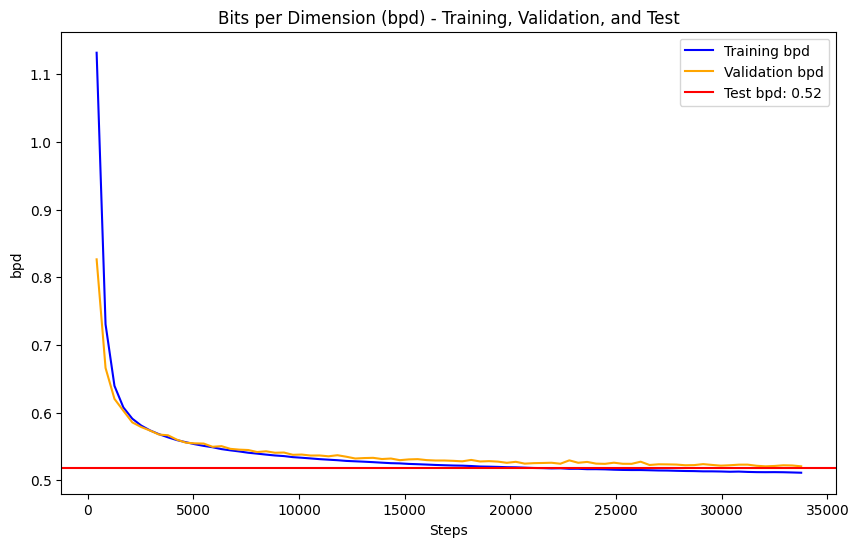
\includegraphics[width=0.8\textwidth]{/Users/ryan/Edu/UvA/Semester1/DL1/DL1-Practicals/assignment3/part1/Results/1-7.png}
    \caption{Training, validation and testing bpd for the VAE}
    \label{fig:VAE_training}
\end{figure}

\subsection{Samples During Training}
\begin{figure}[htbp]
    \centering
    \begin{subfigure}[b]{0.3\textwidth}
        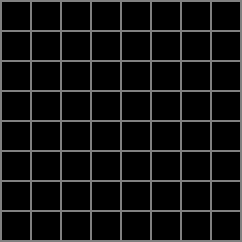
\includegraphics[width=\textwidth]{/Users/ryan/Edu/UvA/Semester1/DL1/DL1-Practicals/assignment3/part1/Results/epoch_0_samples.png}
        \caption{Before Training}
        \label{fig:epoch0}
    \end{subfigure}
    \hfill
    \begin{subfigure}[b]{0.3\textwidth}
        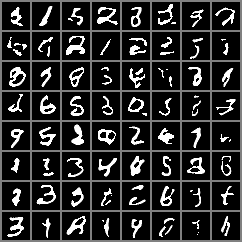
\includegraphics[width=\textwidth]{/Users/ryan/Edu/UvA/Semester1/DL1/DL1-Practicals/assignment3/part1/Results/epoch_10_samples.png}
        \caption{After 10 Epochs}
        \label{fig:epoch10}
    \end{subfigure}
    \hfill
    \begin{subfigure}[b]{0.3\textwidth}
        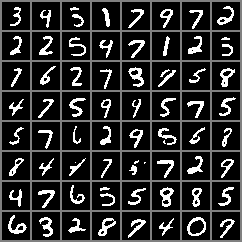
\includegraphics[width=\textwidth]{/Users/ryan/Edu/UvA/Semester1/DL1/DL1-Practicals/assignment3/part1/Results/epoch_80_samples.png}
        \caption{After 80 Epochs}
        \label{fig:epoch80}
    \end{subfigure}
    \caption{Sample Quality Across Training Epochs}
    \label{fig:three_epochs}
\end{figure}
A clear improvement in sample quality can be seen as training progresses. The samples become less blurry and more
closely resemble the human-written digits. Before training the model is not able to generate any meaningful samples
and the images are just noise. After 10 epochs we can see that the model has learned to generate some digits, but
they are quite unrecognisable. For example the 8 might be on its side like an infinity symbol or lines are not finished
and are disconnected. After 80 epochs the model has learned to generate better digits and improves upon the issues
seen after 10 epochs. Still some issues persist like some digits being incomplete like the one seen in row 5 column 3
in Figure 2(c).

\subsection{Manifold}
\bigskip
\newpage

\section{Adverserial Autoencoder Networks}
\subsection{How to compute $q(\mb{z})$ based on different encoders}
In each case, $q(z)$ is computed by integrating over the distribution of $x$ in the dataset, weighted by the encoder's
output distribution $q(z|x)$ for each $x$. The exact form of this integration depends on the nature of the encoder and
the assumed or learned distribution $q(z|x)$.

\subsubsection{$q(\mb{z})$ being a dirac delta function}
In this scenario, the encoder maps each input $x$ to a specific point in the latent space. The overall distribution
$q(z)$ is formed by considering the distribution of $x$ in the data and mapping it through the deterministic function.
If $p(x)$ is the distribution of the data, then $q(z)$ is obtained by integrating over all possible values of $x$:
$$q(z) = \int p(x) \delta(z - f(x)) \, dx$$
Here, $f(x)$ is the deterministic function mapping from $x$ to $z$, and $\delta$ is the Dirac delta function.

\subsubsection{$q(\mb{z})$ being a Gaussian distribution}
For a Gaussian posterior encoder, $q(z)$ is obtained by marginalizing over the distribution of $x$:
$$q(z) = \int p(x) \mathcal{N}(z; \mu(x), \sigma^2(x)) \, dx$$ where $\mu(x)$ and $\sigma(x)$ are the mean and standard
deviation predicted by the encoder for each $x$. This integration considers all possible values of $x$ and their
corresponding Gaussian distributions in the latent space.


\subsubsection{$q(\mb{z})$ being a universal approximator}
In the case of a universal approximator posterior, the computation of $q(z)$ is more complex due to the arbitrary nature
of the distribution $q(z|x)$. The overall distribution $q(z)$ is obtained by integrating over the entire data distribution:
$$q(z) = \int p(x) q(z|x) \, dx$$ where $q(z|x)$ is the complex distribution learned by the encoder for each input $x$.
This integral sums up the contributions of all possible $x$ values to the latent distribution $q(z)$.

\subsection{How do Adversarial Autoencoders reduce the mode collapse problem compared to vanilla GANs}
In vanilla GANs, mode collapse occurs when the generator focuses on producing a limited range of outputs, neglecting the
comprehensive representation of the data distribution. This issue arises because the generator is trained solely based on
the discriminator's feedback, which evaluates the realism of samples without enforcing diversity usually.

In contrast, AAEs incorporate an autoencoder that consists of an encoder and a decoder. The encoder maps input data to
a latent space, while the decoder reconstructs the input from this latent representation. This reconstruction objective
ensures that the latent space captures various aspects of the data, as it needs to accurately reconstruct the original
inputs. Furthermore, the latent space in AAEs is regularized to conform to a predefined prior distribution, commonly
Gaussian. This regularization is achieved through an adversarial process where a discriminator differentiates between
samples from the autoencoder's latent space and those from the target prior distribution.

The training of AAEs balances the reconstruction loss, which promotes data diversity, and the adversarial loss, which
aligns the latent space with the prior distribution. This balance is crucial as it prevents the model from ignoring
significant modes of the data distribution. The diversity in the generated samples is inherently encouraged by the need
for the autoencoder to reconstruct a wide range of input data accurately. Therefore, adversarial auto-encoders mitigate
mode collapse by ensuring diverse representation in the latent space, leading to more varied and representative generated
samples compared to vanilla GANs.

\subsection{Adversarial Autoencoder Training Objective}
\subsubsection{Three Terms of the Formula}
The first term $\mathbb{E}_{p(x)}[\log(1 - D(E(x)))]$ represents the adversarial loss for the discriminator. It
encourages the discriminator $D$ to correctly identify the encoded inputs $E(x)$ as fake. This is part of the
adversarial objective where the encoder $E$ tries to generate latent representations that the discriminator $D$ will
mistakenly classify as coming from the true prior distribution $p(z)$, instead of the data distribution $p(x)$.

The second term $\mathbb{E}_{p(z)}[\log(D(z))]$ encourages the discriminator $D$ to classify the samples $z$ drawn
from the prior distribution $p(z)$ as real.

The third term $\mathbb{E}_{p(x)}[\|x - R(E(x))\|^2]$ is the reconstruction loss, which is part of the reconstruction
objective. It measures the quality of the reconstructed data $R(E(x))$ compared to the original data $x$, using the squared
Euclidean distance as a metric. This term ensures that the autoencoder preserves as much information from the input data as
possible when encoding and decoding.

\subsubsection{Effect of $\lambda$ on the Training Objective}
The hyperparameter $\lambda$ in the adversarial autoencoder training objective balances the importance of the adversarial
loss against the reconstruction loss.
When $\lambda = 1$, the adversarial part of the loss (the terms involving the discriminator $D$) is completely ignored, and
the training objective reduces to solely minimizing the reconstruction loss:
$$ \min_{E, R} \mathbb{E}_{p(x)}\left[\|x - R(E(x))\|^2\right] $$
In this scenario, the autoencoder would focus only on minimizing the difference between the input data and the reconstructed
data. The encoder and decoder would work together to create a representation that allows for accurate reconstruction of the
input data.

On the other hand, when $\lambda = 0$, the reconstruction loss is ignored, and the training objective reduces to only the
adversarial loss:
$$ \min_{E, R} \max_D \mathbb{E}_{p(z)}[\log(D(z))] + \mathbb{E}_{p(x)}[\log(1 - D(E(x)))] $$
In this case, the autoencoder would become an adversarial network that focuses solely on tricking the discriminator into
believing that the outputs of the encoder are from the same distribution as the prior distribution $p(z)$. The encoder would
try to create latent representations of the data that are indistinguishable from samples drawn from the prior distribution
$p(z)$, as judged by the discriminator. However, there would be no incentive for the reconstructed data to resemble the
original input data.

Therefore, $\lambda$ serves as a trade-off parameter that allows one to prioritize between having a good internal
representation that can fool the discriminator (when $\lambda$ is closer to 0) and having a good reconstruction of the input
data (when $\lambda$ is closer to 1). The optimal value of $\lambda$ would typically be somewhere between 0 and 1, balancing
the adversarial and reconstruction aspects of the training objective.

\subsection{Reconstruction Phase}

\subsection{Regularisation Phase}

\subsection{Simple Autoencoder vs Adversarial Autoencoder}

\subsection{Stochastic vs Deterministic Encoder}
A stochastic encoder is beneficial for higher-dimensional latent spaces, such as \( z_{\text{dim}} = 20 \), to avoid
overfitting and enhance the generative capabilities of the model. A deterministic encoder, which maps inputs to fixed points
in the latent space, can lead to a lack of generalization and fail to capture the full complexity of the data distribution,
particularly in higher dimensions. The stochastic encoder introduces variability and regularizes the model by learning
distributions over latent variables. This not only aids in capturing a more nuanced representation of the data but also
encourages a smoother latent space, facilitating the generation of more diverse and representative samples. In contrast,
deterministic approaches may result in a less structured latent space, hindering the AAE's performance, especially when
tasked with generating new data that is both varied and coherent with the training distribution.

\section{Transformers}
\subsection{The Challenge of Long Input Sequence Lengths}
Transformers handle the entire sequence of data simultaneously, thanks to their self-attention mechanism. This design enables
the model to effectively manage dependencies between elements in the sequence, regardless of their distance apart. However,
the challenge arises when dealing with long sequences. The complexity of the self-attention mechanism in Transformers scales
quadratically with the sequence length, both in terms of computation and memory requirements. This makes processing long
sequences resource-intensive and potentially impractical.
To combat this one could introduce sparsity into the attention mechanism, as done in Sparse Transformers. These models
selectively focus on a subset of the input positions per each output position, effectively reducing the overall computational
load. They use a fixed pattern to limit the attention to a subset of the input positions. This approach maintains the essence
of self-attention, allowing the model to focus on the most relevant parts of the input, but they do so in a way that scales
linearly with the sequence length, making them more efficient for processing long sequences.

\subsection{Causal Self-Attention}
\begin{lstlisting}[caption={Causal Self-Attention Forward}, label=lst:causal-self-attention]
    #######################
    # PUT YOUR CODE HERE  #
    #######################
    # Calculate the raw attention scores
    attn_scores = torch.matmul(q, k.transpose(-2, -1))
    
    # Apply the causal mask to ensure that for each position, attention is only applied to the left in the input sequence
    attn_scores = attn_scores.masked_fill(self.mask[:,:,:seq_len,:seq_len] == 0, float('-inf'))
    
    # Normalize the attention scores
    attn_weights = F.softmax(attn_scores, dim=-1)
    
    # Apply dropout to the attention weights
    attn_weights = self.attn_dropout(attn_weights)
    
    # Apply the attention weights to the values
    y = torch.matmul(attn_weights, v)
    #######################
    # END OF YOUR CODE    #
    #######################
\end{lstlisting}

\subsection{Generate Function}
\begin{lstlisting}[caption={GPT Class Generate Function}, label=lst:generate]
    #######################
    # PUT YOUR CODE HERE  #
    #######################
    # Forward the model to get the logits
    logits = self(idx_cond)[:, -1, :]

    # Scale the logits by temperature
    logits = logits / temperature

    # Apply top-k filtering if specified
    if top_k is not None:
        indices_to_remove = logits < torch.topk(logits, top_k)[0][..., -1, None]
        logits[indices_to_remove] = -float('Inf')

    # Convert logits to probabilities
    probabilities = F.softmax(logits, dim=-1)

    # Sampling or choosing the most likely token
    if do_sample:
        next_token = torch.multinomial(probabilities, num_samples=1)
    else:
        next_token = torch.argmax(probabilities, dim=-1, keepdim=True)

    # Append the next token to the sequence
    idx = torch.cat((idx, next_token), dim=-1)
    #######################
    # END OF YOUR CODE    #
    #######################
    \end{lstlisting}
\end{document}